\chapter{Introduction}

This document is intended to describe the main steps required for the integration and configuration of
RTA-SUM LNM module. 
\ifnum \DocumentGroup=1
{
General guidelines on the common steps and workflow for RTA-SUM integration can be found in RTA-SUM Getting Started Guide.
}
\else
{
%Nothing
}\fi

\section{Definitions and Abbreviations}
\label{section:Definitions}
\input{generated/tables/definitions.tex}

\section{Module Overview}
\label{section:overview}
The RTA-SUM LNM, LIN Network Manager, is a software composition located in the Application Layer of the standardized architecture of AUTOSAR, as depicted in Figure \ref{fig:lnm}.


LNM manages interaction with the BSW services related to LIN Network Management for an ECU that is a commander of any LIN Network. There is one LNM per network. So for example, if an ECU is the LIN Commander for three LIN networks, then that ECU must implement three standalone LNM software compositions which each control one LIN network.


LNM is responsible for the following functions:
\begin{itemize}
\item LNM interfaces with the BSW services to track and control the activation status (Full Comm or No Comm) of the LIN Network.
\item LNM interfaces with the BSW services to track and switch the LIN Schedule(s).
\item Collection of all input signals and input integrity signals (e.g. availability from SSM) that are relevant to switching the LIN Schedule(s) for each LIN Network in which the ECU is the LIN Commander. (Integrity signals apply to both the hardware and communication based signals.)
\item Collection of all conditional logic related to activation rules where LIN Network activation criteria is a set of condition linked together.
\item Collection of all conditional logic related to switching the LIN Schedule(s) for each LIN Network in which the ECU is the LIN Commander.
\item Execute the logic to switch the LIN Schedules for each LIN Network in which the ECU is the LIN Commander.
\item Enable the LIN Network when enabled by SUSD
\item Perform the sequence necessary to put the LIN Network to sleep and notify SUSD
\item Detect U codes for Node Loss detection of LIN Responders to ERRH
\item Support Diagnostics of Functional Capability (B Codes, P Codes) via notification to ERRH e.g.: Calibration Download- APPINFO3 (as config), SOH of Responder ECU:APPINFO4
\item Interface with Dcm to receive any required DID requests relevant to the MSCL
\item Interface with Dcm to receive any required RID requests relevant to switching the LIN schedule (i.e. tester initiated relearn of configuration)
\item Calibration Download Support Feature
\item Responder Requested Wakeup Handling
\item MSCL Information: Determine nodes on the bus.
\item Request to BswM to switch the LIN Schedules for the LIN Network.
\item Request to BswM to wake up or put to sleep the LIN Network
\end{itemize}

\begin{figure}[h!]
\begin{center}
	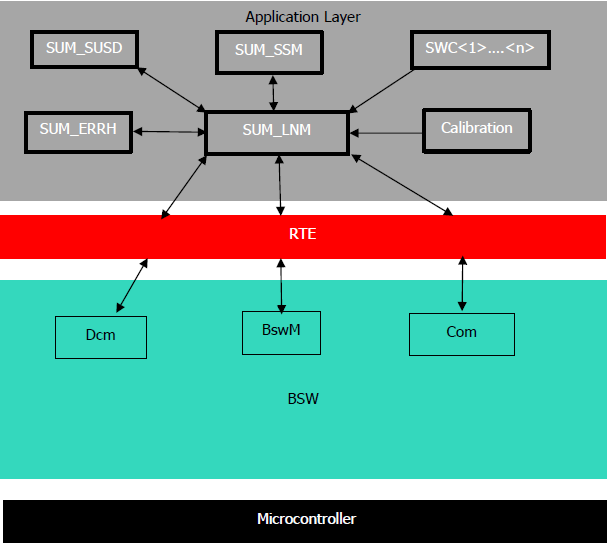
\includegraphics[scale=1]{images/block.png}
  \caption{RTA-SUM LNM Interactions}
  \label{fig:lnm}
\end{center}
\end{figure}

\newpage
\section{References}
\label{sec:ref}
\input{generated/tables/references.tex}

\newpage
\section{User Guide Revision History}
\input{generated/tables/rev_history.tex}